
\subsection{Berechnung der Diffusionsspannung \todo{1x}}\label{k3:diffusion}
Feldst\"arke (Poissongleichung) integrieren und die Skizzen von pn-\"Ubergang, elektrischer
Feldst\"arke und Spannungsverlauf.\\
Siehe \Cref{k5:rlz}.

\subsection{Alle Gleichungen (2x Stromgleichung, 2x Kontinuitätsgleichung, 1x Poisson-Gleichung) \todo{1x}}\label{k3:alleGleichungen}

\subsection{Dotieren \todo{0x}}\label{k3:dotieren}
Dotieren beschreibt den gezielten einbau von Fremdatomen um Ladungstr\"ager zu erzeugen, wodurch die Leitf\"ahigkeit eines
Halbleiters ver\"andert wird (siehe \Cref{fig:dotieren}). Es kommt zu einer unterschiedlichen Konzentration aus Elektronen bzw. L\"ochern und es wird
nun von einem extrinsischem Halbleiter gesprochen.\\
\begin{figure}[h]
    \centering
    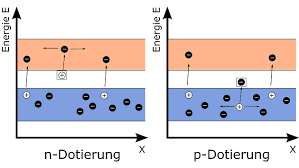
\includegraphics[width=0.4\textwidth]{fig/dotieren}
    \caption{B\"andermodell für n- und p-Dotierung}
    \label{fig:dotieren}
\end{figure}
Durch Dotierung werden Energieniveaus im verbotenen Band erzeugt. Ein Fremdatom aus der 5. Spalte des periodischen Systems
der Elemente wie z.B. P, As oder Sb erzeugt ein Energieniveau in der unmittelbaren Nachbarschaft der Unterkante $E_C$ des
Leitungsbandes. Dieses Energieniveau entsteht dadurch, dass das 5.Valenzelektron der äußersten Schale nicht an der
Bindung im Kristallgitter teilnimmt. Deshalb kann dieses Elektron bereits durch geringfügige Energiezufuhr vom oatierungsatom
abgelöst und in das Leitungsband gehoben werden, wo es sich als Leitungselektron frei bewegt.
Allerdings bleibt zufolge der Ablösung des negativen Elektrons am Dotieratom eine ortsfeste positive Ladung übrig. Die
Ladungen der Dotieratome können selbstverständlich nicht zum Stromtransport beitragen, spielen aber eine wichtige Rolle in
Halbleiterbauelementen.\\
Man nennt einen mit Akzeptoren dotierten Halbleiter kurz p-Halbleiter, den mit Donatoren dotierten n-Halbleiter.

\subsection{Verlauf der Ladungstr\"agerkonzentration als Funktion der Temperatur \todo{0x}}\label{k3:ladungstraegerkonz}
\Cref{fig:fermi}.

\begin{figure}[H]
    \centering
    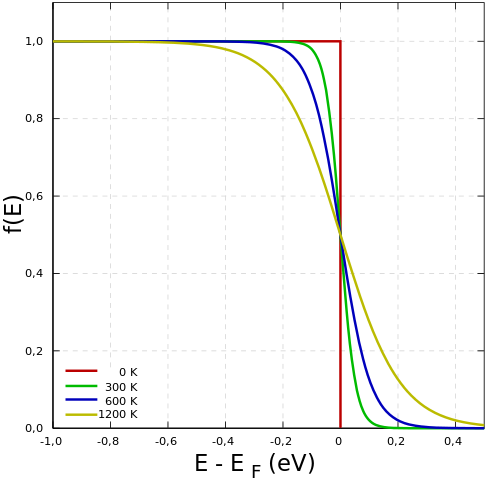
\includegraphics[width=0.4\textwidth]{fig/fermi}
    \caption{Ladungstr\"agerkonzentration bei verschiedenen Temperaturen (\Cref{fig:fermi})}
    \label{fig:fermi2}
\end{figure}

\subsection{Drude Modell \todo{0x}}\label{k3:drude}

Das Drude Modell ist eine klassische Beschreibung des Ladungstransports durch ein externes elektrisches Feld in Metallen.

Im Drude-Modell wird ein elektrischer Leiter als Ionenkristall betrachtet, in dem sich die Elektronen frei bewegen können, ein Elektronengas bilden und so verantwortlich für die Stromleitung sind. Der Begriff Elektronengas rührt von der Ähnlichkeit dieser Theorie zur kinetischen Gastheorie her: herrscht im Inneren des Leiters nämlich kein elektrisches Feld, so verhalten sich die Elektronen wie Gasteilchen in einem Behälter.

Durch ein äußeres elektrisches Feld $\vec {E}$ erfahren die freien Elektronen im Leiter eine Kraftwirkung $F_{el} = q \cdot E$ und werden beschleunigt, jedoch nicht kontinuierlich. Wäre dies so, dann dürften der Widerstand und die Stromstärke nicht konstant sein und das ohmsche Gesetz würde somit nicht gelten. Nach kurzer Zeit stellt sich jedoch ein Gleichgewicht ein, bei dem die mittlere Geschwindigkeit des Elektrons und damit der elektrische Strom proportional zur Feldstärke ist.

Dies wird vom Drude-Modell dadurch erklärt, dass das Elektron mit einem Gitterion zusammenstößt und abgebremst wird. Dieser Vorgang wird phänomenologisch durch eine mittlere Stoßzeit $\tau$ zwischen zwei Kollisionen beschrieben. Mit steigender Temperatur sinkt die mittlere Stoßzeit und damit auch die elektrische Leitfähigkeit der Metalle.

Die Bewegungsgleichung hierfür lautet:
\begin{equation}
    m \dot v + \frac{m}{\tau} v_D = -eE
\end{equation}
mit
\begin{itemize}
    \item $m$ der Elektronenmasse
    \item $v$ der Elektronengeschwindigkeit
    \item $v_D$ der Driftgeschwindigkeit (e-Geschwindigkeit abzüglich der thermischen Geschwindigkeit) und
    \item $\tau$ der Stoßzeit
    \item $e$ der Elementarladung.
\end{itemize}
Für den stationären Zustand $\dot v=0$ gilt:
\begin{equation}
    v_D = -\frac{e\cdot \tau}{m}E
\end{equation}
Mit der Ladungsträgerdichte $n$ n ergibt sich die Stromdichte $j$ damit zu:
\begin{equation}
    j = -e \cdot n \cdot v_D = \frac{e^2 \cdot \tau \cdot n}{m}E
\end{equation}
Die Leitfähigkeit $\sigma$ ist daher:
\begin{equation}
    \sigma = \frac{j}{E} = \frac{e^2 \cdot \tau \cdot n}{m}
\end{equation}

Diese Gleichung wird auch als Drude-Formel oder Drude-Leitfähigkeit bezeichnet. 

\subsection{Hall-Effekt \todo{0x}}\label{k3:halleffekt}
Metallplatte aufzeichnen mit Koordinatensystem und I, B, und F bzw. E als Vektoren.
Kurz beschreiben was im p-HL und n-HL passiert.
Erk\"aren warum der Strom nur in eine Richtung flie{\ss}en kann.

Hall Effekt wird verwendet um Magnetfelder oder Ladungsträgerart (Elektronen oder L\"ocher) und deren Dichte zu bestimmen.
Eine Metallplatte unter spannung wird in des Magnetfeld gestellt.
Das Magnetfeld bewirkt durch die Lorentzkraft eine ablekung der Elektronen senkrecht zur technischen Stromrichtung.
Es kommt zu einer Ladungstrennung (Elektronen und Löcher werden getrennt), die zu einem elektrischen Feld führt (entgegen der
Lorentzkraft). Die so entstandene Spannung lässt sich leicht abgreifen und dadurch kann man das Magnetfeld bestimmen
(\Cref{fig:hall}).

Die Hall-Spannung folgt Strom- und Magnetfeldänderungen in der Regel unmittelbar. Sie steigt mit dem Magnetfeld linear an und ist antiproportional zur (vorzeichenbehafteten) Ladungsträgerdichte[1], da eine geringere Anzahl von Ladungsträgern nur bei höherer Geschwindigkeit der Einzelladungen zu einer unveränderten Stromstärke führen kann. Auf die schnelleren Ladungsträger wirkt eine höhere Lorentz-Kraft, wodurch die Hall-Spannung größer wird. Da die Ladungsträgerdichte in Halbleitern bedeutend kleiner ist als in Metallen, werden vorwiegend Halbleiter als Hall-Sonden benutzt.

\begin{figure}[H]
    \centering
    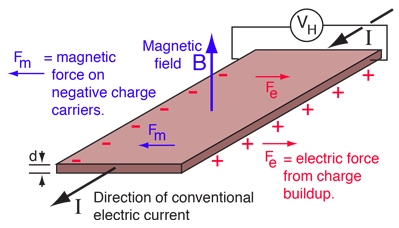
\includegraphics[width=0.4\textwidth]{fig/hall}
    \caption{Aufbau Hall-Effekt}
    \label{fig:hall}
\end{figure}

\subsection{Hall-Spannung \todo{0x}}\label{k3:hallspannung}

\subsection{Diffusionsstrom \todo{0x}}\label{k3:diffusionsstrom}

\subsection{Stromgleichungen \todo{0x}}\label{k3:stromgleichungen}

\subsection{Shockley-Haynes Experiment \todo{0x}}\label{k3:shockleyhaynes}
    \subsubsection{Schlatung aufzeichnen} Oszi und Spannungsquelle nicht vergessen
    \subsubsection{Kurve aufzeichnen und erkl\"aren was abgelesen werden kann}

\subsection{Kontinuit\"atsgleichungen \todo{0x}}\label{k3:kontinuitaet}

	\subsection{Intrinsische Ladungsträgerdichte $n_i$ + Gleichung $n \cdot p=n_i^2$ }
	Die intrinsische Ladungsträgerdichte beschreibt die Eigenleitungsdichte eines Halbleiters. Sie bestimmt den Mindestwert der elektrischen Leitfähigkeit.  
	Bei Halbleitern die auf den absoluten Nullpunkt gekühlt werden, sind alle Elektronen im Kristllgitter gebunden. Erst wenn die Temperatur erhöht wird, können Elektronen durch die nun zur Verfügung stehende thermische Energie vom Valenz- ins Leitungsband gehoben werden.
	Durch Rekombination wandern die Elektronen vom Leitungsband wieder ins Valenzband, dabei wird Energie freigesetzt. 
	Im thermodynamischen Gleichgewicht finden nun Rekombination und Generation von Elektronen statt. Diese sollten im Mittel gleich oft verkommen - um eben ein Gleichgewicht zu erhalten.
	Das bedeutet auch, dass die \textit{Anzahldichte} von freien Elektronen im Mittel konstant ist. 
	Die Eigenleitungsdichte $n_i$ setzt sich also aus der durchschnittlichen Anzahl an freien Elektronen $n$ und Löchern $p$ zusammen. Aufgrund des \textit{Massenwirkungsgesetzes}\footnote{Bei einer reversiblen Reaktion im chemischen Gleichgewicht hat der Quotient aus Ausgangsstoff (Elektron) und Reaktionsprodukt (Loch) einen festen charakteristischen Wert, auch Gleichgewichtskonstante genannt.} kann man schreiben:
	\begin{equation}
	    n_i^2 = n \cdot p
	\end{equation}
	Allerdings ist zu bedenken, dass sich die Eigenleitungsdichte massiv mit der Temperatur verändert, da durch die thermische Energie auch mehr Elektronen im Leitungsband zur Verfügung stehen - das ist auch der Grund warum dotierte Halbleiter ihre typischen Eigenschaften verlieren.
	Zum Beispielt verdoppelt sich $n_i$ bei einem Anstieg von 300 Kelvin auf 310 Kelvin.
	
	Diesen Effekt kann man über folgende Formel beschreiben:
	\begin{equation}
	    n_i^2 = n \cdot p = N_C \cdot N_V e^{-\frac{E_C-E_V}{kT}}
	\end{equation}\label{equ:eigenleitung}
	
	\begin{enumerate}
	    \item $N_C$ ... Bandgewicht des \emph{Leitungsbandes}, also die Zahl der Zustände in $\Delta E$ der Breite kT
	    \begin{enumerate}
	        \item Das Bandgewicht steigt mit der effektiven Masse und mit der Temperatur.
	        \item Höhere Temperatur bedeutet, dass mehr Zustände besetzt sind
	        \item Basiert auf der \textbf{Elektronendichte} $n$
	        \item Wikipedia nennt das die \textbf{Effektive Zustandsdichte} des Leitungsbands
	    \end{enumerate}
	    \item $N_V$ ... Bandgewicht des \emph{Valenzbandes}
	    \begin{enumerate}
	        \item Basiert auf der \textbf{Löcherdichte} $p$
	        \item Wikipedia nennt das die \textbf{Effektive Zustandsdichte} des Valenzbandes
	    \end{enumerate}
	    \item $E_C$ ... Energie der Unterkante des Leitungsbandes
	    \item $E_V$ ... Energie der Oberkante des Valenzbandes
	    \item $k$ ... Boltzmannkonstante
	\end{enumerate}
	
	\begin{enumerate}
	    \item Typische Größen für $n_i$ bei Raumtemperatur (26 Grad, 300 Kelvin)
	    \begin{enumerate}
	        \item Silizium: $1.5 \cdot 10^{10} cm^{-3}$
	        \item Germanium: $2.2 \cdot 10^{13} cm^{-3}$
	    \end{enumerate}
	\end{enumerate}
	
	\subsection{$n_i$ ist Funktion von was? (T und Gap)}
    Wie man in \autoref{equ:eigenleitung} sieht, ist die Eigenleitungsdichte $n_i$ von der Temperatur T abhängig.
    Die Temperaturabhängigkeit verringert sich wenn die Bandlücke, die sich aus $E_G = E_C - E_V$ ergibt, vergrößert. 
    
    Das macht Sinn, denn ein größerer Zähler aus \autoref{equ:eigenleitung} $e^{-\frac{E_G}{kT}}$ kaschiert Änderungen in der Temperatur besser.
    
    \subsubsection{Eigenleitung und Fermi-Niveau}
    Es soll noch erwähnt werden, dass die Eigenleitung $n_i^2$ auch zur Berechnung des Fermi-Niveaus herangezogen werden kann.
    Durch Lösen nach $n_i^2$ von \autoref{equ:eigenleitung} auf und einsetzen in andere Gleichungen kann man das Fermi-Niveau $E_F$ bestimmen bzw. auch zur Berechnung von \textit{p} und \textit{n} heranziehen. 
    Grundaussage ist aber, dass $E_F$ bei Eigenleitung in der Mitte des verbotenen Bandes liegt.
    